\section{HASIL YANG DIHARAPKAN}

\subsection{Hasil yang Diharapkan dari Penelitian}

Dari penelitian yang akan dilakukan, diharapkan mampu menambah wawasan penulis dalam merancang alat anemometer ultrasonic serta
menambahkan penelitian mengenai Raspberry Pi Pico yang saat ini masih jarang ditemukan di kampus ITS.

\subsection{Hasil Pendahuluan}

Telah dilakukan percobaan untuk menganalisa
sinyal pulsa yang diterima dari sensor Ultrasonic US-100. Percobaan dilakukan menggunakan alat Logic Analyser dari Saleae. Kemudian hasil dari logic analyser dibandingkan dengan output yang muncul pada 
serial Raspberry Pi Pico.

\begin{figure}[h!]
	\centering
	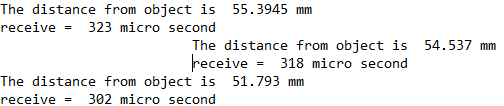
\includegraphics[width=0.7\linewidth]{gambar/serial5cm}
	\caption{Output Serial pada jarak 5cm}
	\label{fig:serial5cm}
\end{figure}
\begin{figure}[h!]
	\centering
	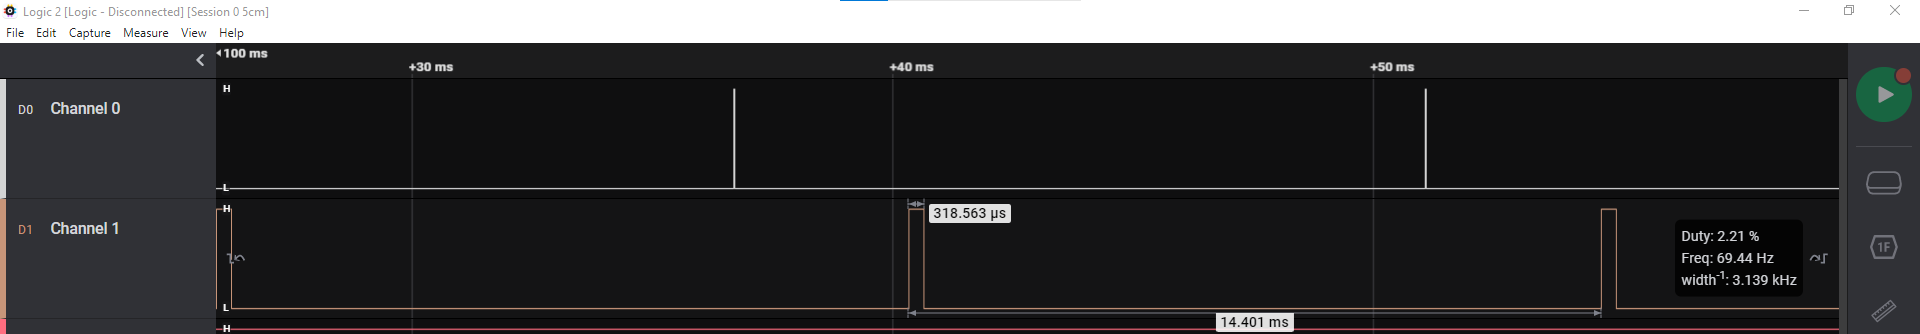
\includegraphics[width=\linewidth]{gambar/logic5cm}
	\caption{Output Sinyal Digital pada jarak 5cm}
	\label{fig:logic5cm}
\end{figure}

Pada percobaan pertama dilakukan pengukuran pada jarak 5 cm. Hasil dari sensor ultrasonic pada output 
serial dapat dilihat pada gambar \ref{fig:serial5cm}. Hasilnya berupa jarak yang terukur 54.537 mm atau 5.46 cm dengan \textit{ToF} 318 mikrosekon. Berikutnya pada logic analyser didapatkan pengukuran 
delta waktu sebesar 318.563 mikrosekon yang dapat dilihat pada gambar \ref{fig:logic5cm}.


\begin{figure}[h!]
	\centering
	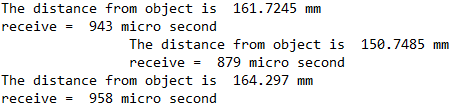
\includegraphics[width=0.7\linewidth]{gambar/serial15cm}
	\caption{Output Serial pada jarak 15cm}
	\label{fig:serial15cm}
\end{figure}
\begin{figure}[h!]
	\centering
	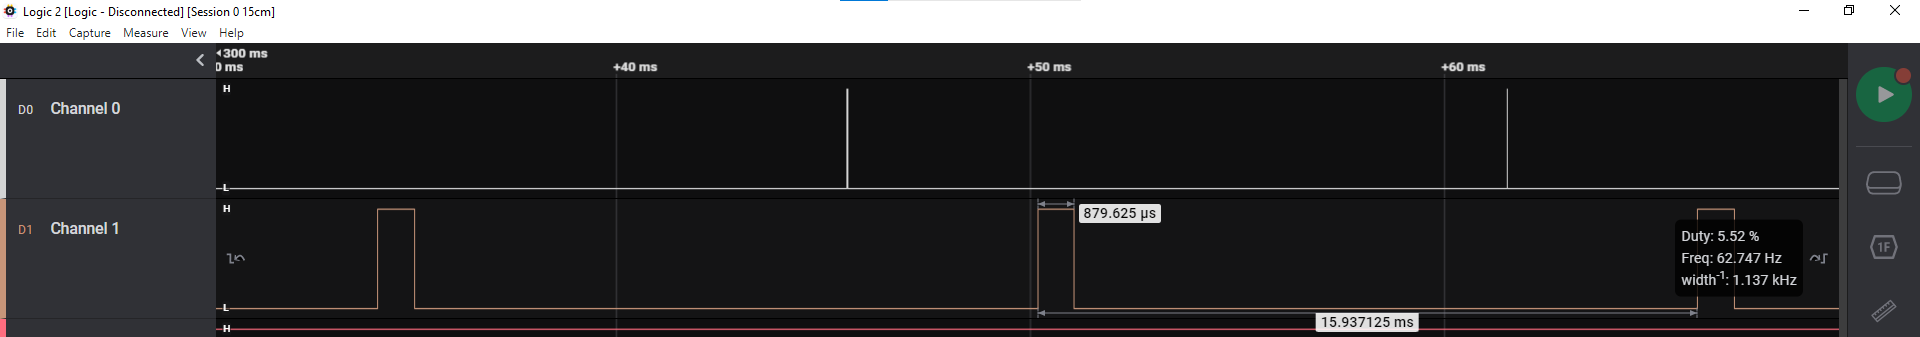
\includegraphics[width=\linewidth]{gambar/logic15cm}
	\caption{Output Sinyal Digital pada jarak 15cm}
	\label{fig:logic15cm}
\end{figure}

Pada percobaan kedua dilakukan pengukuran pada jarak 15 cm. Hasil dari sensor ultrasonic pada output 
serial dapat dilihat pada gambar \ref{fig:serial15cm}. Hasilnya berupa jarak yang terukur 150.7485 mm atau 15.75 cm dengan \textit{ToF} 879 mikrosekon. Berikutnya pada logic analyser didapatkan pengukuran 
delta waktu sebesar 879.625 mikrosekon yang dapat dilihat pada gambar \ref{fig:logic15cm}.


\begin{figure}[h!]
	\centering
	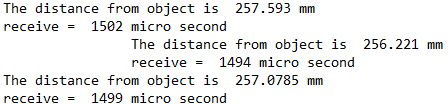
\includegraphics[width=0.7\linewidth]{gambar/serial25cm}
	\caption{Output Serial pada jarak 25cm}
	\label{fig:serial25cm}
\end{figure}
\begin{figure}[h!]
	\centering
	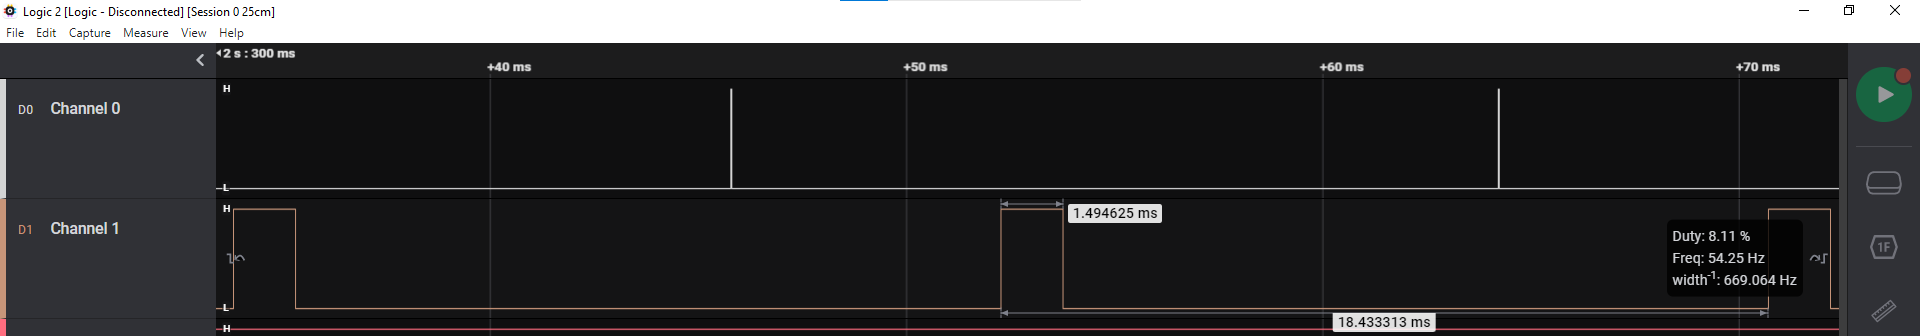
\includegraphics[width=\linewidth]{gambar/logic25cm}
	\caption{Output Sinyal Digital pada jarak 25cm}
	\label{fig:logic25cm}
\end{figure}

Pada percobaan ketiga dilakukan pengukuran pada jarak 25 cm. Hasil dari sensor ultrasonic pada output 
serial dapat dilihat pada gambar \ref{fig:serial25cm}. Hasilnya berupa jarak yang terukur 256.221 mm atau 25.62 cm dengan \textit{ToF} 1494 mikrosekon. Berikutnya pada logic analyser didapatkan pengukuran 
delta waktu sebesar 1494.625 mikrosekon atau 1.494 milisekon yang dapat dilihat pada gambar \ref{fig:logic25cm}.


